\documentclass[tikz,border=10pt]{standalone}
\usepackage{tikz}
\usetikzlibrary{angles, quotes}

\begin{document}
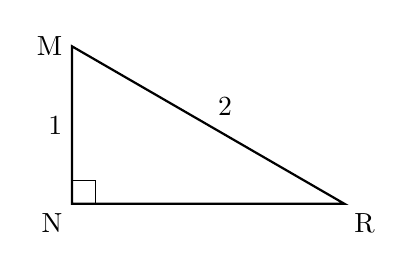
\begin{tikzpicture}[scale=1]

    % Define the coordinates based on the proportions
    % MN = 1, MR = 2 (Hypotenuse)
    % Using Pythagoras: NR = sqrt(2^2 - 1^2) = sqrt(3) approx 1.732
    \coordinate (N) at (0,0);
    \coordinate (M) at (0,2);
    \coordinate (R) at (3.46,0); % Scaled to maintain visual proportions

    % Draw the triangle segments
    \draw[thick] (M) -- (N) -- (R) -- cycle;

    % Draw the right angle symbol at N
    \draw (0,0.3) -- (0.3,0.3) -- (0.3,0);

    % Add labels for the vertices
    \node[below left] at (N) {N};
    \node[left] at (M) {M};
    \node[below right] at (R) {R};

    % Add the measurements/labels exactly as shown
    % Label '1' on the side MN
    \node[left] at (0,1) {1};

    % Label '2' on the hypotenuse MR
    \node[above right] at (1.73, 1) {2};

\end{tikzpicture}
\end{document}
